\chapter{Algorithms}\label{chap:algorithms}
In the following the three load balancing algorithms under test are presented. Firstly, the classic Push-Pull Sum algorithm and the Contiunous Single-Proposal Deal-Agreement-Based Algorithm are introduces. The novel algorithm that is proposed in this paper, the Adaptive Threshold Push-Pull Sum algorithm is then introduced, and it is depicted how the algorithm is composed of the other two algorithms, and why the protocol is composed like that. For all algorithms the pseudo-code and a description of how the algorithms work is presented. Furthermore, example are provided to enhance the understanding of how the algorithms balance load. For the Adaptive Threshold Push-Pull Sum Protocol additionaly the aspired outcome is presented.

\section{Classic Push-Pull Sum Protocol}\label{sec:classicPPS}
The Push-Pull Sum algorithm as proposed in \cite{nugroho2023PushPullSumDataAg} requires each node to have sum $s_{i,r}$ and weight $w_{i,r}$ values as information. The initial weight $w_{i,0}$ for each node is equal to 1. The sum of all weights is equal to the network size $N$. The sum of $s_{i,0}$ is equal to whatever the required input $x_i \in \mathbb{R}^{+}_{0}$ is, in the paper the values for the sums are uniformly distributed values between 0 and 100 \cite{nugroho2023PushPullSumDataAg}. The pseudo code is to be found in figure \ref{alg:PPS}. The Push-Pull Sum algorithm is composed of three different procedures, namely the \textit{RequestData} procedure, the \textit{ResponseData} procedure and the \textit{Aggregate} procedure. In every round $r$ the \textit{Aggregate} procedure is called, except for the first round, since there is no information to be aggregated. In this procedure, every node gatheres all incoming messages $M{node,r}$ sent by other nodes $\{(s_m, w_m)\}$ in the previous round $r-1$, requesting data. Also, nodes update their sum values which essentially is $\sum_{m \in M_{node,r}}{s_m}$ and weight values $\sum_{m \in M_{node,r}}{w_m}$. And finally these values are form the respective load values by dividing sum by weight. Following that, each node calls the \textit{RequestData} procedure. In this procedure, each node chooses a random neighbor node and sends half of its sum $\frac{s_{node,r}}{2}$ and half of its weight $\frac{w_{node,r}}{2}$ to the chosen node and itself. This is the push mechanism. The pull mechanism is described in the \textit{ResponseData} procedure. Here, each node gathers the incoming requests per round $r$ in a set $R_{node, r}$. Then, each node replies to each requesting node (including itself) with the half of its sum value divided by the number of incoming requests, so $\frac{\frac{s_{node,r}}{2}}{|R_{node, r}|}$.

\renewcommand{\algorithmicrequire}{\textbf{Input:}}
\renewcommand{\algorithmicensure}{\textbf{Output:}}
\begin{algorithm}[]
\caption{Push-Pull Sum algorithm}\label{alg:PPS}
\begin{algorithmic}[1]
\Procedure{RequestData}{}
\State Chose a random neighbor node $v$
\State Send $(\frac{s_{u,r}}{2}, \frac{w_{u,r}}{2})$ to the chosen node $v$ and the node $u$ itself
\EndProcedure
\Procedure{ResponseData}{}
\State $R_{u,r} \leftarrow$ Set of the nodes calling $u$ at a round $r$
\For{\textbf{all} $i \in R_{u,r}$}
\State Reply to i with $\left( \frac{\frac{s_{u,r}}{2}}{|R_{u,r}|}, \frac{\frac{w_{u,r}}{2}}{|R_{u,r}|} \right)$
\EndFor
\EndProcedure
\Procedure{Aggregate}{}
\State $M_{u,r} \leftarrow \{(s_{m}, w_{m})\}$ messages sent to $u$ at a round $r-1$
\State $s_{u,r} \leftarrow \sum_{m \in M_{u,r}}^{}s_{m}, w_{u,r} \leftarrow\sum_{m \in M_{u,r}}^{}w_{m}$
\State $f_{avg} \leftarrow \frac{s_{u,r}}{w_{u,r}}$
\EndProcedure
\end{algorithmic}
\end{algorithm}


The Push-Pull Sum algorithm has the mass-conservation property \cite{nugroho2023PushPullSumDataAg}. This property ensures that the values will converge to the same value but not the correct aggregate of the ground truth. They converge to the true mean. The setting in that paper is similar to ours. While they only inspect a complete graph with $10^{4}$ nodes, we have network sizes of $2^{10}$ nodes and more topologies under test. 50 experiments each conducted for 30 rounds were performed. The paper showed that the Push-Pull Sum protocol decreases the expected potential $\Phi_r$ exponentially. The potential function is defined as $\Phi_t=\sum_{i,j}\left(v_{i,j,r}-\frac{w_{i,r}}{n}\right)^{2}$. The $v_{i,j,r}$ component stores the fractional value of node $j$'s contribution at round $r$. The conditional expectation of $\Phi_r+1$ for the Push-Pull Sum protocol is $\mathbb{E}[\Phi_r+1|\Phi_r=\phi]=(\frac{2e-1}{4e}-\frac{1}{4n})\phi$ \cite{nugroho2023PushPullSumDataAg}.

The Push-Pull Sum protocol seemed to perform very well for the complete graph, the Ring of Cliques with large clique size and Lollipop graphs with large clique size, and the star graph. For the star graph the internal node acts as a distributor of the load. While every leaf chooses with 100\% possibility the internal node as a "random" neighbor the internal node is involved as a endpoint of $n-1$ external push operations, and redistributes the load via pull operations to the leaves, where the sum is $\frac{\frac{s_{i,r}}{2}}{n-1}$ and accordingly the weight is $\frac{\frac{w_{i,r}}{2}}{n-1}$. A different explanation applies for the Complete graph, the Ring of Cliques and the Lollipop graph, where the density of each node plays an crucial role. Nodes choose a random neighbor, since the dense graphs have many edges. Randomly choosing a neighbor allows the algorithm to spread loads effectively without relying on a deterministic path, reducing the likelihood of bottlenecks or overloading a single node. That is the reason, why the Push-Pull Sum algorithm did not perform so well for the Torus Grid graph and the Ring graph, where the number of edges is limited to $4$ and $2$ respectively. Here bottlenecks may occur, since two nodes may push back and fourth, with the sum being $\frac{s_{i,r}}{2}$ and the weight being $\frac{w_{i,r}}{2}$, eventhough the load of the nodes may already been averaged and better options for load transfers are ignored due to the lack of determinism.
\subsection{Example}\label{subsec:examplePPS}

\section{Contiunous Single-Proposal Deal-Agreement-Based Protocol}\label{sec:singleproposalDAB}
The Continuous Single-Proposal Algorithm Deal-Agreement-Based algorithm proposed by \cite{Dinitz2023DAB}, is unlike the Push-Pull Sum protocol not an diffusion-based load balancing algorithm. The goal of load balancing is achieved based on deterministic deal-agreements, where one node proposes node to one neighboring node and the neighboring node either accepts transfer proposal in either full or partialy. Dinitz et al. algorithm is a anytime algorithm, as they never the worsen the state of the network during execution. They can be stopped at \textit{any time} of the execution. They studied the algorithm in a dynamic setting, which means that the graph may experience changes between rounds. Furthermore, the algorithm is a localized one, where the nodes only work with the information regarding the load state of themselves and their neighbors load state. Each node has a set of neighboring nodes and their including the node's initial load itself as initial information. The algorithm is divided into three phases. There is the \textit{proposal}, \textit{deal} and the \textit{summary}-phase. In the \textit{proposal}-phase each node $u$ contacts the minimal loaded neighbor \textit{v} and sends a proposal to that neighbor, if the neighbor is less loaded. The proposal is of value $(\frac{load_{r}(u)-load_{r}(v)}{2})$, which is labeled as a \textit{fair} proposal. Since the load transfer is fair, the resulting load of $u$ is not lower than that of $v$. Following that, the nodes enter the \textit{deal}-phase. In this phase nodes evaluate the deals proposed to them. A node accepts the deal of the node that proposes the maximal load transfer. The actual transfer happens and the load values are being updated. Finally, in the \textit{summary}-phase each node informs their neighbors regarding their updated load values. \cite{Dinitz2023DAB}
\renewcommand{\algorithmicrequire}{\textbf{Input:}}
\renewcommand{\algorithmicensure}{\textbf{Output:}}
\begin{algorithm}
\caption{Continuous Single-Proposal Deal-Agreement-Based protocol}\label{alg:DAB}
\begin{algorithmic}[1]
\Require An undirected graph $G=(V,E,load)$
\Ensure A load state with discrepancy at most $\epsilon$ on $G$
\For{$r=1$ and on}
\For{every node u}
\State Find a neighbor, $v$, with the minimal load
\If{$load_{r}(u) - load_{r}(v)>0$}
\State $u$ sends to $v$ a transfer proposal of value $(load_{r}(u)-load_{r}(v))/2$
\EndIf
\EndFor

\For{every node $u$}
\If{there is at least one transfer proposal to $u$}
\State Find a neighbor, $w$, proposing to $u$ the maximal transfer
\State Node $u$ makes a deal: informs node $w$ on accepting its proposal
\State The actual transfer from $w$ to $u$ is executed 
\EndIf
\EndFor

\For{every node $u$}
\State Node $u$ sends the updated value of its load to its neighbors
\EndFor
\EndFor
\end{algorithmic}
\end{algorithm}

The analysis in this paper is based on a potential function. Dinitz et al. defines potential for a node $u$ as $p(u) = (load(u)-L_{avg})^{2}$ where $L_{avg}$ is the current load average in the network. The potential for the Graph $p(G)$ is defined as $p(G)=\sum_{u\in V}{p(u)}$, which essentially is the sum of all potential of each node in the graph G. Any fair load transfer of load $l$ decreases the potential of the graph by at least $2*l^{2}$. And as a result of any round $r$ of the Contiunous Single-Proposal Deal-Agreement-Based Protocol, the graph potential decreases by at least $\frac{K^{2}_r}{2D_r}$ where $K$ is the initial discrepancy and $D$ is a bound for the graph diameter. \cite{Dinitz2023DAB}

The Single-Proposal Deal-Agreement-Based load balancing algorithm seems to have difficulties in reducing the mean squared error as rapidly as the Push-Pull Sum algorithm for dense graphs like the a complete graph, the Lollipop graph with large clique size, the ring of cliques with large clique sizes. This seems to be the case, since each node is looking for a minimal load partner. For a complete graph the minimal load partner are the same nodes with same loads equal to the minimal load of the network. This causes each node to propose to the same node with $L_{min}$ which then evaluates the proposals, and accepts exactly one transfer proposal, namely the maximal one. An analouge scenario happens for the Ring of Cliques and Lollipop graph, with the difference that for the Ring of Cliques not each node is proposing to the same minimal neighbor, but for the minimal laoded neighbor within their respective cliques. For the Lollipop graph, the nodes in the path graph balance their loads more quickly than the nodes in the clique which is a bottleneck in this scenario. Looking at the Torus Grid graph and the Ring graph, this Deal-Agreement-Based protocol seems to perform very well in reducing the error, since the proposals are more distributed for the nodes due to the density of the graph, and thus more nodes are involved in load transfers. The star graph makes an exception to this case, since we have a similar bottleneck as in the complete graph, where the internal node is the common neighbor for each leaf and thus each leaf proposes load to the internal node. The internal node, then chooses only the maximal proposing transfer. The simulation results in the student project \cite{Bayazitoglu} indicate the performances of each load balancing algorithm for each topology very clearly.
\subsection{Example}\label{subsec:exampleDAB}
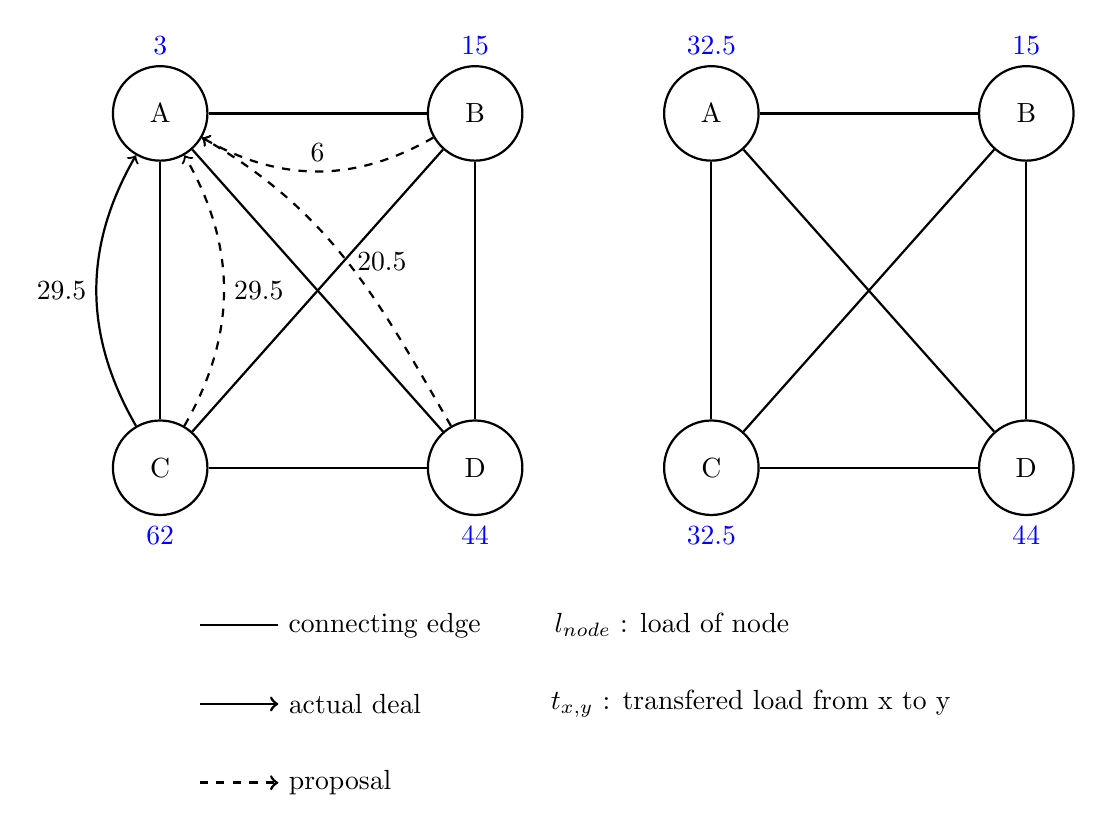
\begin{tikzpicture}[ thick, main node/.style={circle, draw, minimum size=1.2cm}]

    % First graph
    \node[main node] (A1) at (0.5,4.5) {A};
    \node[main node] (B1) at (4.5,4.5) {B};
    \node[main node] (C1) at (0.5,0) {C};
    \node[main node] (D1) at (4.5,0) {D};
    
    \node[above, color=blue] at (A1.north) {3};
    \node[above, color=blue] at (B1.north) {15};
    \node[below, color=blue] at (C1.south) {62};
    \node[below, color=blue] at (D1.south) {44};
    
    \draw (A1) -- (B1);
    \draw (A1) -- (C1);
    \draw (A1) -- (D1);
    \draw (B1) -- (C1);
    \draw (B1) -- (D1);
    \draw (C1) -- (D1);

    % Second graph
    \node[main node] (A2) at (7.5,4.5) {A};
    \node[main node] (B2) at (11.5,4.5) {B};
    \node[main node] (C2) at (7.5,0) {C};
    \node[main node] (D2) at (11.5,0) {D};
    
    \node[above, color=blue] at (A2.north) {32.5};
    \node[above, color=blue] at (B2.north) {15};
    \node[below, color=blue] at (C2.south) {32.5};
    \node[below, color=blue] at (D2.south) {44};
    
    \draw (A2) -- (B2);
    \draw (A2) -- (C2);
    \draw (A2) -- (D2);
    \draw (B2) -- (C2);
    \draw (B2) -- (D2);
    \draw (C2) -- (D2);

    \draw[->] (C1) to[out=120, in=240] node[left] {$29.5$} (A1);
    \draw[dashed, ->] (C1) to[out=60, in=300] node[right] {$29.5$} (A1);
    \draw[dashed, ->] (B1) to[out=210, in=330] node[above] {$6$} (A1);
    \draw[dashed, ->] (D1) to[out=120, in=330] node[right] {$20.5$} (A1);

    % Legend in the middle below the graphs
    \begin{scope}[shift={(3,-2)}]
        % Horizontal line
        \draw (-2,0) -- (-1,0) node[right] {connecting edge};
        % Long right arrow
        \draw[->, line width=1pt] (-2,-1) -- (-1,-1) node[right] {actual deal};
        % Long right dashed arrow
        \draw[->, dashed, line width=1pt] (-2,-2) -- (-1,-2) node[right] {proposal};
        
        % Load notation
        \node at (4,0) {$l_{node}$ : load of node};
        \node at (5,-1) {$t_{x,y}$ : transfered load from x to y};
    \end{scope}

\end{tikzpicture}
\todo{See section 1.1 of Dinitz paper to describe to methods of load balancing fot the DAB.}

\section{Adaptive Threshold Push-Pull Sum Protocol}\label{sec:adaptivethresholdPPS}
The Adaptive Threhsold Push-Pull Sum algorithm is composed of different ideas and elements of the two former algorithms, extended by the idea of adaptive thresholding. The Adaptive Threshold Push-Pull Sum consits of different procedures. In the \textit{CheckThresholdsRequestData} each node $i$ chooses a subset $RN$ of $\log_{2}{(|neighborhood|)}$ random neighbors. This is to enhance the chance of a good load transfer to happen. If we only choose one neighbor the chance is lower to find an optimal or good neighbor to execute a load transfer. Then the load difference between the node $i$ and each node in $RN$ is computed and checked if the load difference is bigger than some threshold $\theta$. The threshold is computed in the \textit{CalculateThresholds}-procedure. The threshold $\theta$ is computed as $k*\sqrt{MSE_r-1}$ where $k$ is some factor to adjust the sensitivity of the threshold. A larger $k$ means the threshold is more sensitive meaning that less nodes are eligiable for load transfer and vice versa. This condition prevents load transfers with low effect, and guarantees a selection of nodes with effect above the given threshold. The first eligiable node receives the sum and the weight in form of a push action $(\frac{s_i,r}{2})$ for the sum and $(\frac{w_i,r}{2})$ for the weight. The \textit{ResponseData}, and the \textit{Aggregate}-procedure are analoge to the classic Push-Pull Sum algorithm. The push and the pull mechanism are directly taken from the Push-Pull Sum algorithm, thus the name Adaptive Threshold Push-Pull Sum algorithm. Two ideas are derived from the Single-Proposal Deal-Agreement-Based algorithm. The idea of the conditional load transfer is analog to the Single-Proposal Deal-Agreement-Based's one, with the only difference that the difference of load between the two negotiating nodes shouldn't be larger than $0$, but bigger than a threshold $\theta$. And instead of initiaing a load transfer with the maximal loaded node, the Adaptive Threshold Push-Pull Sum algorithm orders the nodes to initiate a load transfer with the first node proposing load. The reason for that is that we want to avoid that each node looks through the whole set $R_n$ and needs to evaluate each proposal, instead the first node proposing a load transfer is accepted as a transfer partner.
\begin{algorithm}
    \caption{Adaptive Threshold Push-Pull Sum algorithm}\label{alg:PPS}
    \begin{algorithmic}[1]
    \Procedure{CalculateThresholds}{}
    \State $\theta \leftarrow k * \sqrt{MSE_{r-1}}$ 
    \EndProcedure
    \Procedure{CheckTresholdRequestData}{}
    \State $RN_{u,r} \leftarrow$ choose $\lceil \log_{2}{(|neighborhood(u)|)} \rceil$ random neighbor
    \For{every node $v_{i} \in RN_{u,r}$}
    \State $\Delta_{u, v_{i}} \leftarrow |(load(u) - load(v_{i}))|$
    \If{$\Delta_{u,v} > \theta$}
    \State Send $(\frac{s_{u,r}}{2}, \frac{w_{u,r}}{2})$ to first node v fulfilling condition and the node $u$ itself
    \EndIf
    \EndFor
    \EndProcedure
    \Procedure{ResponseData}{}
    \State $R_{u,r} \leftarrow$ Set of the nodes calling $u$ at a round $r$
    \For{\textbf{all} $i \in R_{u,r}$}
    \State Reply to i with $\left( \frac{\frac{s_{u,r}}{2}}{|R_{u,r}|}, \frac{\frac{w_{u,r}}{2}}{|R_{u,r}|} \right)$
    \EndFor
    \EndProcedure
    \Procedure{Aggregate}{}
    \State $M_{u,t} \leftarrow \{(s_{m}, w_{m})\}$ messages sent to $u$ at a round $r-1$
    \State $s_{u,t} \leftarrow \sum_{m \in M_{u,r}}^{}s_{m}, w_{u,r} \leftarrow\sum_{m \in M_{u,r}}^{}w_{m}$
    \State $load(u) \leftarrow \frac{s_{u,r}}{w_{u,r}}$
    \EndProcedure
    \end{algorithmic}
    \end{algorithm}
\subsection{Example}\label{subsec:exampleAdaptiveThresholdPPS}
\subsection{Aspired Outcome}\label{subsec:aspiredOutcomeAdaptiveThresholdPPS}
Thinking of the simulation results presented in \cite{Bayazitoglu} the discrepancy between the MSE reduction per round for the different topologies show that the algorithms perform either very well or medicore to bad. The main idea and perspective designing this algorithm was to find a compromise solution to that, to provide a better adaptability for different network topologies.
